
\chap{四元数代数}
\section{介绍}
本章包含进一步的历史背景,四元数的发明,并涵盖四元数代数的演变。我展示了如何通过将四元数视为有序对来极大地简化四元数代数,并提供了加法、减法、实数、纯四元数和单位四元数的示例。在定义了复共轭、范数、四元数积、平方和逆之后,我将展示如何用矩阵表示四元数。本章最后总结了重要的定义和几个工作实例。



\section{一些历史}
Hamilton 定义了一个四元数$q$,它的相关规则为
$$
    q=s+i a+j b+k c, \quad s, a, b, c \in \mathbb{R}
$$
其中,
$$
    \begin{gathered}
        i^{2}=j^{2}=k^{2}=i j k=-1 \\
        i j=k, \quad j k=i, \quad k i=j \\
        j i=-k, k j=-i, i k=-j
    \end{gathered}
$$
引用\cite{bib6-1,bib6-2,bib6-3} 但我们倾向于将四元数写成
$$
    q=s+a i+b j+c k
$$
从 Hamilton 的规则中观察$i  j$的出现是如何被$k$所取代的。额外的虚数k项是循环模式$i j=k, j k=i$和$k i=j$的关键,它们非常类似于两个单位笛卡尔矢量的叉乘:
$$
    \mathbf{i} \times \mathbf{j}=\mathbf{k}, \quad \mathbf{j} \times \mathbf{k}=\mathbf{i}, \quad \mathbf{k} \times \mathbf{i}=\mathbf{j} .
$$
事实上,这种相似性并非巧合,因为 Hamilton 也发明了标量和向量乘积。然而,尽管四元数提供了一个描述向量的代数框架,人们必须承认,在 Hamilton 之前,向量已经被研究了很多年。

Hamilton 还发现$i, j, k$项可以表示三个笛卡尔单位向量$\mathbf{i}, \mathbf{j}$和$\mathbf{k}$,它们必须具有虚数性质。例如$\mathbf{i}^{2}=-1$,等等,这对于一些数学家和科学家来说不太好,他们怀疑是否有必要涉及这么多虚项。

汉密尔顿寻找复数的三维等效物的动机部分是代数的,部分是几何的。因为如果一个复数是由有序对表示的,并且能够以$90^{\circ}$旋转平面上的点,那么也许一个三元组可以以$90^{\circ}$旋转空间中的点。最后,一个三元组必须被一个四元组-一个四元数取代。

我们可以从两个角度来看待 Hamilton 的规则。首先,它们是三个虚项组合的代数结果。第二,它们反映了一个潜在的空间几何结构。后一种解释被P. G. Tait(p.g.泰特)所采用,并在他的《四元数的基本论述》一书中进行了概述。Tait的方法假设三个单位向量$\mathbf{i}, \mathbf{j}$, $\mathbf{k}$分别与$x$-, $y$-, $z$-轴对齐:

\begin{CJK}{UTF8}{gkai}
    $\mathbf{i}$与$\mathbf{j}$相乘的结果或$\mathbf{ij}$定义为$\mathbf{j}$在垂直于$\mathbf{i}$的平面上沿正方向转动一个直角,换句话说,$\mathbf{i}$对$\mathbf{j}$的操作将其翻转过来,使其与$\mathbf{k}$重合;因此简而言之$\mathbf{i} \mathbf{j}=\mathbf{k}$。

    为了保持一致,必须承认,如果$\mathbf{i}$不是对$\mathbf{j}$进行操作,而是对平面$y z$中垂直于$\mathbf{i}$的任何其他单位向量进行操作,它将使其在同一方向上经过一个直角,因此$\mathbf{i k}$只能是$-\mathbf{j}$。

    将我们引用$\mathbf{i}$来说明的定义扩展到其他单位向量,很明显,$\mathbf{j}$对$\mathbf{k}$的运算必须使其转回$\mathbf{i}$,或$\mathbf{j} \mathbf{k}=\mathbf{i}$。。\cite{bib6-4}
\end{CJK}

其解释如图\ref{fig:6-1} a-d所示。图\ref{fig:6-1}a显示了 $\mathbf{i}$, $\mathbf{j}$, $\mathbf{k}$的原始对齐方式。图\ref{fig:6-1}b显示了 $\mathbf{j}$ 转动 $\mathbf{k}$ 的效果。图\ref{fig:6-1}c显示了 $\mathbf{k}$ 转动 $\mathbf{i}$,图6.1d显示了 $\mathbf{i}$ 转动 $\mathbf{j}$。

\begin{figure}[htbp]
    \centering
    \subfigure[]{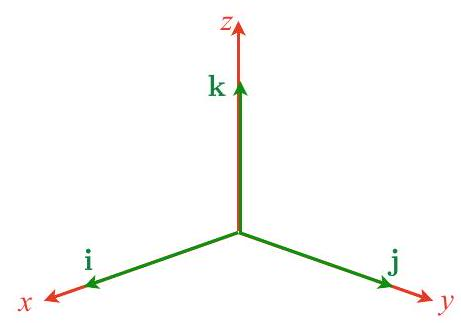
\includegraphics[max width=0.3\textwidth]{2023_04_20_41f1ceac5a31dc7d1b59g-089(1)}}
    \subfigure[]{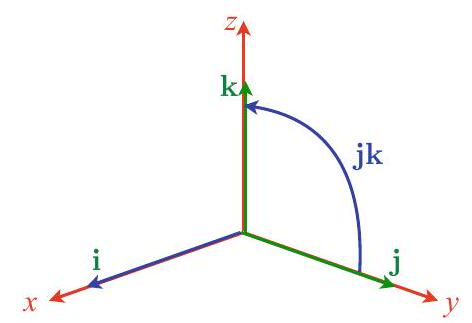
\includegraphics[max width=0.3\textwidth]{2023_04_20_41f1ceac5a31dc7d1b59g-089(2)}}\\
    \subfigure[]{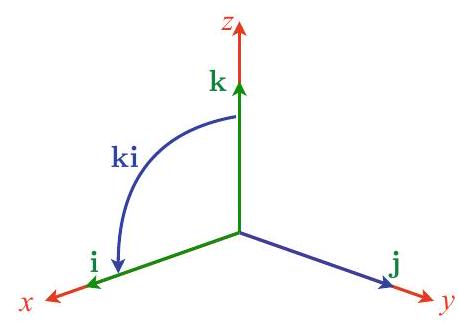
\includegraphics[max width=0.3\textwidth]{2023_04_20_41f1ceac5a31dc7d1b59g-089}}
    \subfigure[]{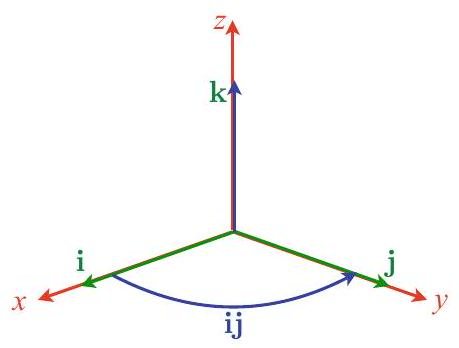
\includegraphics[max width=0.3\textwidth]{2023_04_20_41f1ceac5a31dc7d1b59g-089(3)}}
    \caption[short]{ 解释乘积$\mathbf{j k,  ki, ij}$}
    \label{fig:6-1}
\end{figure}


到目前为止,还没有提到虚数——我们只有:
$$
    \begin{aligned}
         & \mathbf{i j}=\mathbf{k}, \quad \mathbf{j k}=\mathbf{i}, \quad \mathbf{k i}=\mathbf{j} \\
         & \mathbf{j i}=-\mathbf{k}, \mathbf{k j}=-\mathbf{i}, \mathbf{i k}=-\mathbf{j} .
    \end{aligned}
$$

如果我们假设这些向量服从代数的分配律和结合律,它们的虚性质就暴露出来了。例如:
$$
    \mathbf{i j}=\mathbf{k}
$$

然后以$\mathbf{i}$相乘:
$$
    \mathbf{i i j}=\mathbf{i k}=-\mathbf{j}
$$

因此,
$$
    \mathbf{i i}=\mathbf{i}^{2}=-1
$$

同样,我们可以展示 $\mathbf{j}^{2}=\mathbf{k}^{2}=-1$.

接下来:

$$
    \mathbf{i} \mathbf{j} \mathbf{k}=\mathbf{i}(\mathbf{j} \mathbf{k})=\mathbf{i} \mathbf{i}=\mathbf{i}^{2}=-1
$$

因此,仅仅通过声明叉积的作用, Hamilton 的规则就出现了,带有所有虚数的特征。它还提出了下列意见:


A very curious speculation, due to Servois, and published in 1813 in Gergonne's Annales is the only one, so far has been discovered, in which the slightest trace of an anticipation of Quaternions is contained. Endeavouring to extend to space the form $a+b \sqrt{-1}$ for the plane, he is guided by analogy to write a directed unit-line in space the form

$$
    p \cos \alpha+q \cos \beta+r \cos \gamma
$$

where $\alpha, \beta, \gamma$ are its inclinations to the three axes. He perceives easily that $p, q, r$ must be non-reals : but, he asks, "seraient-elles imaginaires réductibles à la forme générale $A+B \sqrt{-1}$ ?" This could not be the answer. In fact they are the $\mathbf{i}, \mathbf{j}, \mathbf{k}$ of the Quaternion Calculus. [4]

So the French mathematician François-Joseph Servois (1768-1847), was another person who came very close to discovering quaternions. Furthermore, both Tait and Hamilton were apparently unaware of the paper published by Rodrigues.

And it doesn't stop there. The brilliant German mathematician Carl Friedrich Gauss (1777-1855), was extremely cautious, and nervous of publishing anything too revolutionary, just in case he was ridiculed by fellow mathematicians. His diaries reveal that he had anticipated non-euclidean geometry ahead of Nikolai Ivanovich Lobachevsky. And in a short note from his diary in 1819 [5] he reveals that he had identified a method of finding the product of two quadruples $(a, b, c, d)$ and $(\alpha, \beta, \gamma, \delta)$ as:

$$
    \begin{aligned}
        (A, B, C, D)= & (a, b, c, d)(\alpha, \beta, \gamma, \delta)                               \\
        =             & (a \alpha-b \beta-c \gamma-d \delta, a \beta+b \alpha-c \delta+d \gamma   \\
                      & a \gamma+b \delta+c \alpha-d \beta, a \delta-b \gamma+c \beta+d \alpha) .
    \end{aligned}
$$

At first glance, this result does not look like a quaternion product, but if we transpose the second and third coordinates of the quadruples, and treat them as quaternions, we have:

$$
    \begin{aligned}
        (A, B, C, D) & =(a+c i+b j+d k)(\alpha+\gamma i+\beta j+\delta k)                                    \\
                     & =a \alpha-c \gamma-b \beta-d \delta+a(\gamma i+\beta j+\delta k)                      \\
                     & =+\alpha(c i+b j+d k),(b \delta-d \beta) i+(d \gamma-c \delta) j+(c \beta-b \gamma) k
    \end{aligned}
$$

which is identical to Hamilton's quaternion product! Furthermore, Gauss also realised that the product was non-commutative. However, he did not publish his findings, and it was left to Hamilton to invent quaternions for himself, publish his results and take the credit.

In 1881 and 1884, Josiah Willard Gibbs, at Yale University, printed his lecture notes on vector analysis for his students. Gibbs had cut the 'umbilical cord' between the real and vector parts of a quaternion and raised the 3 -D vector as an independent object without any imaginary connotations. Gibbs also took on board the ideas of the German mathematician Hermann Günter Grassmann (1809-1877), who had been developing his own ideas for a vectorial system since 1832 . Gibbs also defined the scalar and vector products using the relevant parts of the quaternion product. Finally, in 1901, a student of Gibbs, Edwin Bidwell Wilson, published Gibbs' notes in book form: Vector Analysis [6], which contains the notation in use today.

Quaternion algebra is definitely imaginary, yet simply by isolating the vector part and ignoring the imaginary rules, Gibbs was able to reveal a new branch of mathematics that exploded into vector analysis. Hamilton and his supporters were unable to persuade their peers that quaternions could represent vectorial quantities, and eventually, Gibbs' notation won the day, and quaternions faded from the scene.

In recent years, quaternions have been rediscovered by the flight simulation industry, and more recently by the computer graphics community, where they are used to rotate vectors about an arbitrary axis. In the intervening years, various people have had the opportunity to investigate the algebra, and propose new ways of harnessing its qualities.

So let's look at three ways of annotating a quaternion $q$ :

$$
    \begin{aligned}
         & q=s+x i+y j+z k                                                               \\
         & q=s+\mathbf{v}                                                                \\
         & q=[s, \mathbf{v}]                                                             \\
         & \text { wheres, } x, y, z \in \mathbb{R}, \quad \mathbf{v} \in \mathbb{R}^{3} \\
         & \text { and } i^{2}=j^{2}=k^{2}=-1 .
    \end{aligned}
$$

The difference is rather subtle. In (6.1) we have Hamilton's original definition with its imaginary terms and associated rules. In (6.2) a ' + ' sign is used to add a scalar to a vector, which seems strange, yet works. In (6.3) we have an ordered pair comprising a scalar and a vector.

Now you may be thinking: How is it possible to have three different definitions for the same object? Well, I would argue that you can call an object whatever you like, so long as they are algebraically identical. For example, matrix notation is used to represent a set of linear equations, and leads to the same results as every-day equations. Therefore, both systems of notation are equally valid.

Although I have employed the notation in (6.1) and (6.2) in other publications, in this book I have used ordered pairs. So what we need to show is that Hamilton's original definition of a quaternion (6.1), with its scalar and three imaginary terms, can be replaced by an ordered pair (6.3) comprising a scalar and a 'modern' vector.

\section{四元数定义}
Let's start with two quaternions $q_{a}$ and $q_{b}$ à la Hamilton:

$$
    \begin{aligned}
         & q_{a}=s_{a}+x_{a} i+y_{a} j+z_{a} k \\
         & q_{b}=s_{b}+x_{b} i+y_{b} j+z_{b} k
    \end{aligned}
$$

and the obligatory rules:

$$
    \begin{gathered}
        i^{2}=j^{2}=k^{2}=i j k=-1 \\
        i j=k, \quad j k=i, \quad k i=j \\
        j i=-k, k j=-i, i k=-j .
    \end{gathered}
$$

Our objective is to show that $q_{a}$ and $q_{b}$ can also be represented by the ordered pairs

$$
    \begin{aligned}
        q_{a} & =\left[s_{a}, \mathbf{a}\right]                                                                                       \\
        q_{b} & =\left[s_{b}, \mathbf{b}\right], \quad s_{a}, s_{b} \in \mathbb{R}, \quad \mathbf{a}, \mathbf{b} \in \mathbb{R}^{3} .
    \end{aligned}
$$

The quaternion product $q_{a} q_{b}$ expands to

$$
    \begin{aligned}
        q_{a} q_{b}=\left[s_{a}, \mathbf{a}\right]\left[s_{b}, \mathbf{b}\right]= & {\left[s_{a}+x_{a} i+y_{a} j+z_{a} k\right]\left[s_{b}+x_{b} i+y_{b} j+z_{b} k\right] } \\
        =                                                                         & {\left[\left(s_{a} s_{b}-x_{a} x_{b}-y_{a} y_{b}-z_{a} z_{b}\right)\right.}             \\
                                                                                  & +\left(s_{a} x_{b}+s_{b} x_{a}+y_{a} z_{b}-y_{b} z_{a}\right) i                         \\
                                                                                  & +\left(s_{a} y_{b}+s_{b} y_{a}+z_{a} x_{b}-z_{b} x_{a}\right) j                         \\
                                                                                  & \left.+\left(s_{a} z_{b}+s_{b} z_{a}+x_{a} y_{b}-x_{b} y_{a}\right) k\right] .
    \end{aligned}
$$

Equation (6.4) takes the form of another quaternion, and confirms that the quaternion product is closed.

At this stage, Hamilton turned the imaginary terms $i, j, k$ into unit Cartesian vectors $\mathbf{i}, \mathbf{j}, \mathbf{k}$ and transformed (6.4) into a vector form. The problem with this approach is that the vectors retain their imaginary roots. Simon Altmann's suggestion is to replace the imaginaries by the ordered pairs:

$$
    i=[0, \mathbf{i}], \quad j=[0, \mathbf{j}], \quad k=[0, \mathbf{k}]
$$

which are themselves quaternions, and called quaternion units.

The idea of defining a quaternion in terms of quaternion units is exactly the same as defining a vector in terms of its unit Cartesian vectors. Furthermore, it permits vectors to exist without any imaginary associations.

Let's substitute these quaternion units in (6.4) together with $[1, \mathbf{0}]=1$ :

$$
    \begin{aligned}
        {\left[s_{a}, \mathbf{a}\right]\left[s_{b}, \mathbf{b}\right]=} & {\left[\left(s_{a} s_{b}-x_{a} x_{b}-y_{a} y_{b}-z_{a} z_{b}\right)[1, \mathbf{0}]\right.}  \\
                                                                        & +\left(s_{a} x_{b}+s_{b} x_{a}+y_{a} z_{b}-y_{b} z_{a}\right)[0, \mathbf{i}]                \\
                                                                        & +\left(s_{a} y_{b}+s_{b} y_{a}+z_{a} x_{b}-z_{b} x_{a}\right)[0, \mathbf{j}]                \\
                                                                        & \left.+\left(s_{a} z_{b}+s_{b} z_{a}+x_{a} y_{b}-x_{b} y_{a}\right)[0, \mathbf{k}]\right] .
    \end{aligned}
$$

Next, we expand (6.5) using previously defined rules:

$$
    \begin{aligned}
        {\left[s_{a}, \mathbf{a}\right]\left[s_{b}, \mathbf{b}\right]=} & {\left[\left[s_{a} s_{b}-x_{a} x_{b}-y_{a} y_{b}-z_{a} z_{b}, \mathbf{0}\right]\right.}                \\
                                                                        & +\left[0,\left(s_{a} x_{b}+s_{b} x_{a}+y_{a} z_{b}-y_{b} z_{a}\right) \mathbf{i}\right]                \\
                                                                        & +\left[0,\left(s_{a} y_{b}+s_{b} y_{a}+z_{a} x_{b}-z_{b} x_{a}\right) \mathbf{j}\right]                \\
                                                                        & \left.+\left[0,\left(s_{a} z_{b}+s_{b} z_{a}+x_{a} y_{b}-x_{b} y_{a}\right) \mathbf{k}\right]\right] .
    \end{aligned}
$$

A vertical scan of (6.6) reveals some hidden vectors:

$$
    \begin{aligned}
        {\left[s_{a}, \mathbf{a}\right]\left[s_{b}, \mathbf{b}\right]=} & {\left[\left[s_{a} s_{b}-x_{a} x_{b}-y_{a} y_{b}-z_{a} z_{b}, \mathbf{0}\right]\right.}                                                                                      \\
                                                                        & +\left[0, s_{a}\left(x_{b} \mathbf{i}+y_{b} \mathbf{j}+z_{b} \mathbf{k}\right)+s_{b}\left(x_{a} \mathbf{i}+y_{a} \mathbf{j}+z_{a} \mathbf{k}\right)\right.                   \\
                                                                        & \left.\left.+\left(y_{a} z_{b}-y_{b} z_{a}\right) \mathbf{i}+\left(z_{a} x_{b}-z_{b} x_{a}\right) \mathbf{j}+\left(x_{a} y_{b}-x_{b} y_{a}\right) \mathbf{k}\right]\right] .
    \end{aligned}
$$

Equation (6.7) contains two ordered pairs which can now be combined:

$$
    \begin{aligned}
        {\left[s_{a}, \mathbf{a}\right]\left[s_{b}, \mathbf{b}\right]=} & {\left[s_{a} s_{b}-x_{a} x_{b}-y_{a} y_{b}-z_{a} z_{b},\right.}                                                                                                 \\
                                                                        & +s_{a}\left(x_{b} \mathbf{i}+y_{b} \mathbf{j}+z_{b} \mathbf{k}\right)+s_{b}\left(x_{a} \mathbf{i}+y_{a} \mathbf{j}+z_{a} \mathbf{k}\right)                      \\
                                                                        & \left.+\left(y_{a} z_{b}-y_{b} z_{a}\right) \mathbf{i}+\left(z_{a} x_{b}-z_{b} x_{a}\right) \mathbf{j}+\left(x_{a} y_{b}-x_{b} y_{a}\right) \mathbf{k}\right] .
    \end{aligned}
$$

If we make

$$
    \begin{aligned}
         & \mathbf{a}=x_{a} \mathbf{i}+y_{a} \mathbf{j}+z_{a} \mathbf{k} \\
         & \mathbf{b}=x_{b} \mathbf{i}+y_{b} \mathbf{j}+z_{b} \mathbf{k}
    \end{aligned}
$$

and substitute them in (6.8) we get:

$$
    \left[s_{a}, \mathbf{a}\right]\left[s_{b}, \mathbf{b}\right]=\left[s_{a} s_{b}-\mathbf{a} \cdot \mathbf{b}, s_{a} \mathbf{b}+s_{b} \mathbf{a}+\mathbf{a} \times \mathbf{b}\right]
$$

which defines the quaternion product.

From now on, we don't have to worry about Hamilton's rules as they are embedded within (6.9). Furthermore, our vectors have no imaginary associations.

Although Rodrigues did not have access to Gibbs' vector notation used in (6.9), he managed to calculate the equivalent algebraic expression, which was some achievement.

\subsection{四元数单位}
Using (6.9) we can check to see if the quaternion units are imaginary by squaring them:

$$
    \begin{aligned}
        i     & =[0, \mathbf{i}]                                             \\
        i^{2} & =[0, \mathbf{i}][0, \mathbf{i}]                              \\
              & =[\mathbf{i} \cdot \mathbf{i}, \mathbf{i} \times \mathbf{i}] \\
              & =[-1, \mathbf{0}]
    \end{aligned}
$$

which is a real quaternion and equivalent to -1 , confirming that $[0, \mathbf{i}]$ is imaginary. Using a similar expansion we can shown that $[0, \mathbf{j}]$ and $[0, \mathbf{k}]$ have the same property. Now let's compute the products $i j, j k$ and $k i$ :

$$
    \begin{aligned}
        i j & =[0, \mathbf{i}][0, \mathbf{j}]                               \\
            & =[-\mathbf{i} \cdot \mathbf{j}, \mathbf{i} \times \mathbf{j}] \\
            & =[0, \mathbf{k}]
    \end{aligned}
$$

which is the quaternion unit $k$.

$$
    \begin{aligned}
        j k & =[0, \mathbf{j}][0, \mathbf{k}]                               \\
            & =[-\mathbf{j} \cdot \mathbf{k}, \mathbf{j} \times \mathbf{k}] \\
            & =[0, \mathbf{i}]
    \end{aligned}
$$

which is the quaternion unit $i$.

$$
    \begin{aligned}
        k i & =[0, \mathbf{k}][0, \mathbf{i}]                               \\
            & =[-\mathbf{k} \cdot \mathbf{i}, \mathbf{k} \times \mathbf{i}] \\
            & =[0, \mathbf{j}]
    \end{aligned}
$$

which is the quaternion unit $j$.

Next, let's confirm that $i j k=-1$ :

$$
    \begin{aligned}
        \text { ijk } & =[0, \mathbf{i}][0, \mathbf{j}][0, \mathbf{k}]                \\
                      & =[0, \mathbf{k}][0, \mathbf{k}]                               \\
                      & =[-\mathbf{k} \cdot \mathbf{k}, \mathbf{k} \times \mathbf{k}] \\
                      & =[-1, \mathbf{0}]
    \end{aligned}
$$

which is a real quaternion equivalent to -1 , confirming that $i j k=-1$.

Thus the notation of ordered pairs upholds all of Hamilton's rules. However, the last double product assumes that quaternions are associative. So let's double check to show that $(i j) k=i(j k)$ :

$$
    \begin{aligned}
        i(j k) & =[0, \mathbf{i}][0, \mathbf{j}][0, \mathbf{k}]                \\
               & =[0, \mathbf{i}][0, \mathbf{i}]                               \\
               & =[-\mathbf{i} \cdot \mathbf{i}, \mathbf{i} \times \mathbf{i}] \\
               & =[-1, \mathbf{0}]
    \end{aligned}
$$

which is correct.

\subsection{四元数乘积示例}
Although we have yet to discover how quaternions are used to rotate vectors, let's concentrate on their algebraic traits by evaluating an example.

$$
    \begin{aligned}
         & q_{a}=[1,2 \mathbf{i}+3 \mathbf{j}+4 \mathbf{k}] \\
         & q_{b}=[2,3 \mathbf{i}+4 \mathbf{j}+5 \mathbf{k}]
    \end{aligned}
$$

the product $q_{a} q_{b}$ is

$$
    \begin{aligned}
        q_{a} q_{b}= & {[1,2 \mathbf{i}+3 \mathbf{j}+4 \mathbf{k}][2,3 \mathbf{i}+4 \mathbf{j}+5 \mathbf{k}] }                    \\
        =            & {[1 \times 2-(2 \times 3+3 \times 4+4 \times 5),}                                                          \\
                     & 1(3 \mathbf{i}+4 \mathbf{j}+5 \mathbf{k})+2(2 \mathbf{i}+3 \mathbf{j}+4 \mathbf{k})                        \\
                     & +(3 \times 5-4 \times 4) \mathbf{i}-(2 \times 5-4 \times 3) \mathbf{j}+(2 \times 4-3 \times 3) \mathbf{k}] \\
        =            & {[-36,7 \mathbf{i}+10 \mathbf{j}+13 \mathbf{k}-\mathbf{i}+2 \mathbf{j}-\mathbf{k}] }                       \\
        =            & {[-36,6 \mathbf{i}+12 \mathbf{j}+12 \mathbf{k}] }
    \end{aligned}
$$

which is another ordered pair representing a quaternion.

Having shown that Hamilton's imaginary notation has a vector equivalent, and can be represented as an ordered pair, we continue with this notation and describe other features of quaternions. Note that we can abandon Hamilton's rules as they are embedded within the definition of the quaternion product, and will surface in the following definitions.

\section{代数定义}
A quaternion is the ordered pair:

$$
    q=[s, \mathbf{v}], \quad s \in \mathbb{R}, \quad \mathbf{v} \in \mathbb{R}^{3}
$$

If we express $\mathbf{v}$ in terms of its components, we have

$$
    q=[s, x \mathbf{i}+y \mathbf{j}+z \mathbf{k}], \quad s, x, y, z \in \mathbb{R}
$$

\section{四元数加减法}
Addition and subtraction employ the following rule:

$$
    \begin{aligned}
        q_{a}           & =\left[s_{a}, \mathbf{a}\right]                            \\
        q_{b}           & =\left[s_{b}, \mathbf{b}\right]                            \\
        q_{a} \pm q_{b} & =\left[s_{a} \pm s_{b}, \mathbf{a} \pm \mathbf{b}\right] .
    \end{aligned}
$$

For example:

$$
    \begin{aligned}
        q_{a}       & =[0.5,2 \mathbf{i}+3 \mathbf{j}-4 \mathbf{k}]   \\
        q_{b}       & =[0.1,4 \mathbf{i}+5 \mathbf{j}+6 \mathbf{k}]   \\
        q_{a}+q_{b} & =[0.6,6 \mathbf{i}+8 \mathbf{j}+2 \mathbf{k}]   \\
        q_{a}-q_{b} & =[0.4,-2 \mathbf{i}-2 \mathbf{j}-10 \mathbf{k}]
    \end{aligned}
$$

\section{实四元数}
A real quaternion has a zero vector term:

$$
    q=[s, \mathbf{0}]
$$

The product of two real quaternions is

$$
    \begin{aligned}
        q_{a}       & =\left[s_{a}, \mathbf{0}\right]                               \\
        q_{b}       & =\left[s_{b}, \mathbf{0}\right]                               \\
        q_{a} q_{b} & =\left[s_{a}, \mathbf{0}\right]\left[s_{b}, \mathbf{0}\right] \\
                    & =\left[s_{a} s_{b}, \mathbf{0}\right]
    \end{aligned}
$$

which is another real quaternion, and shows that they behave just like real numbers:

$$
    [s, \mathbf{0}] \equiv s
$$

We have already come across this with complex numbers containing a zero imaginary term:

$$
    a+b i=a, \quad \text { when } b=0
$$

\section{四元数乘以标量}
Intuition suggests that multiplying a quaternion by a scalar should obey the rule:

$$
    \begin{aligned}
        q         & =[s, \mathbf{v}]                                      \\
        \lambda q & =\lambda[s, \mathbf{v}], \quad \lambda \in \mathbb{R} \\
                  & =[\lambda s, \lambda \mathbf{v}] .
    \end{aligned}
$$

For example:

$$
    \begin{aligned}
        q & =3[2,3 \mathbf{i}+4 \mathbf{j}+5 \mathbf{k}]    \\
          & =[6,9 \mathbf{i}+12 \mathbf{j}+15 \mathbf{k}] .
    \end{aligned}
$$

We can confirm our intuition by multiplying a quaternion by a scalar in the form of a real quaternion:

$$
    \begin{aligned}
        q         & =\left[\begin{array}{ll}
                s, & \mathbf{v}
            \end{array}\right]                \\
        \lambda   & =[\lambda, \mathbf{0}]                                  \\
        \lambda q & =\left[\begin{array}{ll}
                \lambda, & \mathbf{0}
            \end{array}\right][s, \mathbf{v}] \\
                  & =\left[\begin{array}{ll}
                \lambda s, & \lambda \mathbf{v}
            \end{array}\right]
    \end{aligned}
$$

which is excellent confirmation.

\section{纯四元数}
Hamilton defined a pure quaternion as one having a zero scalar term:

$$
    q=x i+y j+z k
$$

and is just a vector, but with imaginary qualities. Simon Altmann, and others, believe that this was a serious mistake on Hamilton's part to call a quaternion with a zero real term, a vector.

The main issue is that there are two types of vectors: polar and axial, also called a pseudovector. Richard Feynman describes polar vectors as 'honest' vectors [7] and represent the every-day vectors of directed lines. Whereas, axial vectors are computed from polar vectors, such as in a vector product. However, these two types of vector do not behave in the same way when transformed. For example, given two 'honest', polar vectors $\mathbf{a}$ and $\mathbf{b}$, we can compute the axial vector: $\mathbf{c}=\mathbf{a} \times \mathbf{b}$. Next, if we subject $\mathbf{a}$ and $\mathbf{b}$ to an inversion transform through the origin, such that $\mathbf{a}$ becomes $-\mathbf{a}$, and $\mathbf{b}$ becomes $-\mathbf{b}$, and compute their cross product $(-\mathbf{a}) \times(-\mathbf{b})$, we still get c! Which implies that the axial vector $\mathbf{c}$ must not be transformed along with a and $\mathbf{b}$.

It could be argued that the inversion transform is not a 'proper' transform as it turns a right-handed set of axes into a left-handed set. But in physics, laws of nature are expected to work in either system. Unfortunately, Hamilton was not aware of this distinction, as he had only just invented vectors. However, in the intervening years, it has become evident that Hamilton's quaternion vector is an axial vector, and not a polar vector. As we will see, in 3-D rotations quaternions take the form

$$
    q=\left[\cos \left(\frac{\theta}{2}\right), \sin \left(\frac{\theta}{2}\right) \mathbf{v}\right]
$$

where $\theta$ is the angle of rotation and $\mathbf{v}$ is the axis of rotation, and when we set $\theta=180^{\circ}$, we get

$$
    q=[0, \mathbf{v}]
$$

which remains a quaternion, even though it only contains a vector part.

Consequently, we define a pure quaternion as

$$
    q=[0, \mathbf{v}]
$$

The product of two pure quaternions is

$$
    \begin{aligned}
        q_{a}       & =[0, \mathbf{a}]                                              \\
        q_{b}       & =[0, \mathbf{b}]                                              \\
        q_{a} q_{b} & =[0, \mathbf{a}][0, \mathbf{b}]                               \\
                    & =[-\mathbf{a} \cdot \mathbf{b}, \mathbf{a} \times \mathbf{b}]
    \end{aligned}
$$

which is no longer 'pure', as some of the original vector information has 'tunnelled' across into the real part via the dot product.

\section{单位四元数}
Let's pursue this analysis further by introducing some familiar vector notation.

Give vector $\mathbf{v}$, then

$$
    \mathbf{v}=\lambda \hat{\mathbf{v}}, \quad \text { where } \lambda=\|\mathbf{v}\| \text { and }\|\hat{\mathbf{v}}\|=1
$$

Combining this with the definition of a pure quaternion we get:

$$
    \begin{aligned}
        q & =[0, \mathbf{v}]               \\
          & =[0, \lambda \hat{\mathbf{v}}] \\
          & =\lambda[0, \hat{\mathbf{v}}]
    \end{aligned}
$$

and reveals the object $[0, \hat{\mathbf{v}}]$ which is called the unit quaternion and comprises a zero scalar and a unit vector. It is convenient to identify this unit quaternion as $\hat{q}$ :

$$
    \hat{q}=[0, \hat{\mathbf{v}}]
$$

So now we have a notation similar to that of vectors where a vector $\mathbf{v}$ is described in terms of its unit form:

$$
    \mathbf{v}=\lambda \hat{\mathbf{v}}
$$

and a quaternion $q$ is also described in terms of its unit form:

$$
    q=\lambda \hat{q}
$$

Note that $\hat{q}$ is an imaginary object as it squares to -1 :

$$
    \begin{aligned}
        \hat{q}^{2} & =[0, \hat{\mathbf{v}}][0, \hat{\mathbf{v}}]                                           \\
                    & =[-\hat{\mathbf{v}} \cdot \hat{\mathbf{v}}, \hat{\mathbf{v}} \times \hat{\mathbf{v}}] \\
                    & =[-1, \mathbf{0}]                                                                     \\
                    & =-1
    \end{aligned}
$$

which is not too surprising, bearing in mind Hamilton's original invention!

\section{四元数的加法形式}
We now come to the idea of splitting a quaternion into its constituent parts: a real quaternion and a pure quaternion. Again, intuition suggests that we can write a quaternion as

$$
    \begin{aligned}
        q & =[s, \mathbf{v}]                 \\
          & =[s, \mathbf{0}]+[0, \mathbf{v}]
    \end{aligned}
$$

and we can test this by forming the algebraic product of two quaternions represented in this way:

$$
    \begin{aligned}
        q_{a}       & =\left[s_{a}, \mathbf{0}\right]+[0, \mathbf{a}]                                                                                                                                          \\
        q_{b}       & =\left[s_{b}, \mathbf{0}\right]+[0, \mathbf{b}]                                                                                                                                          \\
        q_{a} q_{b} & =\left(\left[s_{a}, \mathbf{0}\right]+[0, \mathbf{a}]\right)\left(\left[s_{b}, \mathbf{0}\right]+[0, \mathbf{b}]\right)                                                                  \\
                    & =\left[s_{a}, \mathbf{0}\right]\left[s_{b}, \mathbf{0}\right]+\left[s_{a}, \mathbf{0}\right][0, \mathbf{b}]+[0, \mathbf{a}]\left[s_{b}, \mathbf{0}\right]+[0, \mathbf{a}][0, \mathbf{b}] \\
                    & =\left[s_{a} s_{b}, \mathbf{0}\right]+\left[0, s_{a} \mathbf{b}\right]+\left[0, s_{b} \mathbf{a}\right]+[-\mathbf{a} \cdot \mathbf{b}, \mathbf{a} \times \mathbf{b}]                     \\
                    & =\left[s_{a} s_{b}-\mathbf{a} \cdot \mathbf{b}, s_{a} \mathbf{b}+s_{b} \mathbf{a}+\mathbf{a} \times \mathbf{b}\right]
    \end{aligned}
$$

which is correct, and confirms that the additive form works.

\section{四元数的双体形式}
Having shown that the additive form of a quaternion works, and discovered the unit quaternion, we can join the two objects together as follows:

$$
    \begin{aligned}
        q & =[s, \mathbf{v}]                              \\
          & =[s, \mathbf{0}]+[0, \mathbf{v}]              \\
          & =[s, \mathbf{0}]+\lambda[0, \hat{\mathbf{v}}] \\
          & =s+\lambda \hat{q} .
    \end{aligned}
$$

Just to recap, $s$ is a scalar, $\lambda$ is the length of the vector term, and $\hat{q}$ is the unit quaternion $[0, \hat{\mathbf{v}}]$.

Look how similar this notation is to a complex number:

$$
    \begin{aligned}
         & z=a+b i             \\
         & q=s+\lambda \hat{q}
    \end{aligned}
$$

where $a, b, s, \lambda$ are scalars, $i$ is the unit imaginary and $\hat{q}$ is the unit quaternion.

\section{四元数的复共轭}
We have already discovered that the conjugate of a complex number $z=a+b \mathrm{i}$ is given by

$$
    z^{*}=a-b \mathrm{i}
$$

and is very useful in computing the inverse of $z$. The quaternion conjugate plays a similar role in computing the inverse of a quaternion. Therefore, given

$$
    q=[s, \mathbf{v}]
$$

the quaternion conjugate is defined as

$$
    q^{*}=[s,-\mathbf{v}]
$$

For example:

$$
    \begin{aligned}
        q     & =[2,3 \mathbf{i}-4 \mathbf{j}+5 \mathbf{k}]  \\
        q^{*} & =[2,-3 \mathbf{i}+4 \mathbf{j}-5 \mathbf{k}]
    \end{aligned}
$$

If we compute the product $q q^{*}$ we obtain

$$
    \begin{aligned}
        q q^{*} & =[s, \mathbf{v}][s,-\mathbf{v}]                                                                             \\
                & =\left[s^{2}-\mathbf{v} \cdot(-\mathbf{v}),-s \mathbf{v}+s \mathbf{v}+\mathbf{v} \times(-\mathbf{v})\right] \\
                & =\left[s^{2}+\mathbf{v} \cdot \mathbf{v}, \mathbf{0}\right]                                                 \\
                & =\left[s^{2}+v^{2}, \mathbf{0}\right] .
    \end{aligned}
$$

Let's show that $q q^{*}=q^{*} q$ :

$$
    \begin{aligned}
        q^{*} q & =[s,-\mathbf{v}][s, \mathbf{v}]                                                                               \\
                & =\left[s^{2}-(-\mathbf{v}) \cdot \mathbf{v}, s \mathbf{v}-s \mathbf{v}+(-\mathbf{v}) \times \mathbf{v}\right] \\
                & =\left[s^{2}+\mathbf{v} \cdot \mathbf{v}, \mathbf{0}\right]                                                   \\
                & =\left[s^{2}+v^{2}, \mathbf{0}\right]                                                                         \\
                & =q q^{*}
    \end{aligned}
$$

Now let's show that $\left(q_{a} q_{b}\right)^{*}=q_{b}^{*} q_{a}^{*}$.

$$
    \begin{aligned}
        q_{a}                        & =\left[s_{a}, \mathbf{a}\right]                                                                                         \\
        q_{b}                        & =\left[s_{b}, \mathbf{b}\right]                                                                                         \\
        q_{a} q_{b}                  & =\left[s_{a}, \mathbf{a}\right]\left[s_{b}, \mathbf{b}\right]                                                           \\
                                     & =\left[s_{a} s_{b}-\mathbf{a} \cdot \mathbf{b}, s_{a} \mathbf{b}+s_{b} \mathbf{a}+\mathbf{a} \times \mathbf{b}\right]   \\
        \left(q_{a} q_{b}\right)^{*} & =\left[s_{a} s_{b}-\mathbf{a} \cdot \mathbf{b},-s_{a} \mathbf{b}-s_{b} \mathbf{a}-\mathbf{a} \times \mathbf{b}\right] .
    \end{aligned}
$$

Next, we compute $q_{b}^{*} q_{a}^{*}$

$$
    \begin{aligned}
        q_{a}^{*}           & =\left[s_{a},-\mathbf{a}\right]                                                                                         \\
        q_{b}^{*}           & =\left[s_{b},-\mathbf{b}\right]                                                                                         \\
        q_{b}^{*} q_{a}^{*} & =\left[s_{b},-\mathbf{b}\right]\left[s_{a},-\mathbf{a}\right]                                                           \\
                            & =\left[s_{a} s_{b}-\mathbf{a} \cdot \mathbf{b},-s_{a} \mathbf{b}-s_{b} \mathbf{a}-\mathbf{a} \times \mathbf{b}\right] .
    \end{aligned}
$$

And as (6.10) equals $(6.11),\left(q_{a} q_{b}\right)^{*}=q_{b}^{*} q_{a}^{*}$.

\section{四元数的范数}
The norm of a complex number $z=a+b i$ is defined as:

$$
    |z|=\sqrt{a^{2}+b^{2}}
$$

which allows us to write

$$
    z z^{*}=|z|^{2}
$$

Similarly, the norm of a quaternion $q$ is defined as:

$$
    \begin{aligned}
        q   & =[s, \mathbf{v}]               \\
            & =[s, \lambda \hat{\mathbf{v}}] \\
        |q| & =\sqrt{s^{2}+\lambda^{2}}
    \end{aligned}
$$

where $\lambda=\|\mathbf{v}\|$ which allows us to write

$$
    q q^{*}=|q|^{2}
$$

For example:

$$
    \begin{aligned}
        q   & =[1,4 \mathbf{i}+4 \mathbf{j}-4 \mathbf{k}] \\
        |q| & =\sqrt{1^{2}+4^{2}+4^{2}+(-4)^{2}}          \\
            & =\sqrt{49}                                  \\
            & =7
    \end{aligned}
$$

\section{归一化四元数}
A quaternion with a unit norm is called a normalised quaternion. For example, the quaternion $q=[s, \mathbf{v}]$ is normalised by dividing it by $|q|$ :

$$
    q^{\prime}=\frac{q}{\sqrt{s^{2}+\lambda^{2}}}
$$

We must be careful not to confuse the unit quaternion with a unit-norm quaternion. The unit quaternion is $[0, \hat{\mathbf{v}}]$ with a unit-vector part, whereas a unit-norm quaternion is normalised such that $s^{2}+\lambda^{2}=1$.

I will be careful to distinguish between these two terms as many authorsincluding myself-use the term unit quaternion to describe a quaternion with a unit norm. For example:

$$
    q=[1,4 \mathbf{i}+4 \mathbf{j}-4 \mathbf{k}]
$$

has a norm of 7 , and $q$ is normalised by dividing by 7 :

$$
    q^{\prime}=\frac{1}{7}[1,4 \mathbf{i}+4 \mathbf{j}-4 \mathbf{k}]
$$

The type of unit-norm quaternion we will be using takes the form:

$$
    q=\left[\cos \left(\frac{\theta}{2}\right), \sin \left(\frac{\theta}{2}\right) \hat{\mathbf{v}}\right]
$$

because $\cos ^{2} \theta+\sin ^{2} \theta=1$

\section{四元数乘积}
Having shown that ordered pairs can represent a quaternion and its various manifestations, let's summarise the products we will eventually encounter. To start, we have the product of two normal quaternions:

$$
    \begin{aligned}
        q_{a} q_{b} & =\left[s_{a}, \mathbf{a}\right]\left[s_{b}, \mathbf{b}\right]                                                           \\
                    & =\left[s_{a} s_{b}-\mathbf{a} \cdot \mathbf{b}, s_{a} \mathbf{b}+s_{b} \mathbf{a}+\mathbf{a} \times \mathbf{b}\right] .
    \end{aligned}
$$

\subsection{纯四元数的乘积}
Given two pure quaternions:

$$
    \begin{aligned}
         & q_{a}=[0, \mathbf{a}] \\
         & q_{b}=[0, \mathbf{b}]
    \end{aligned}
$$

their product is

$$
    \begin{aligned}
        q_{a} q_{b} & =[0, \mathbf{a}][0, \mathbf{b}]                                 \\
                    & =[-\mathbf{a} \cdot \mathbf{b}, \mathbf{a} \times \mathbf{b}] .
    \end{aligned}
$$

\subsection{两个归一化四元数的乘积}
Given two unit-norm quaternions:

$$
    \begin{aligned}
         & q_{a}=\left[s_{a}, \mathbf{a}\right] \\
         & q_{b}=\left[s_{b}, \mathbf{b}\right]
    \end{aligned}
$$

where $\left|q_{a}\right|=\left|q_{b}\right|=1$. Their product is another unit-norm quaternion, which is proved as follows.

We assume $q_{c}=\left[s_{c}, \mathbf{c}\right]$ and show that $\left|q_{c}\right|=s_{c}^{2}+c^{2}=1$ where

$$
    \begin{aligned}
        {\left[s_{c}, \mathbf{c}\right] } & =\left[s_{a}, \mathbf{a}\right]\left[s_{b}, \mathbf{b}\right]                                                           \\
                                          & =\left[s_{a} s_{b}-\mathbf{a} \cdot \mathbf{b}, s_{a} \mathbf{b}+s_{b} \mathbf{a}+\mathbf{a} \times \mathbf{b}\right] .
    \end{aligned}
$$

Let's assume the angle between $\mathbf{a}$ and $\mathbf{b}$ is $\theta$, which permits us to write:

$$
    \begin{aligned}
         & s_{c}=s_{a} s_{b}-a b \cos \theta                                                                                        \\
         & \mathbf{c}=s_{a} b \hat{\mathbf{b}}+s_{b} a \hat{\mathbf{a}}+a b \sin \theta(\hat{\mathbf{a}} \times \hat{\mathbf{b}}) .
    \end{aligned}
$$

Fig. 6.2 Geometry for $s_{a} b \hat{\mathbf{b}}+s_{b} a \hat{\mathbf{a}}+a b \sin \theta(\hat{\mathbf{a}} \times$ b)

\begin{center}
    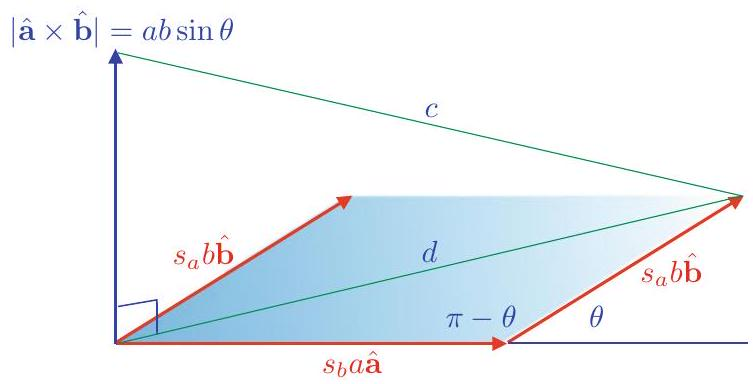
\includegraphics[max width=\textwidth]{2023_04_20_41f1ceac5a31dc7d1b59g-104}
\end{center}

Therefore,

$$
    \begin{aligned}
        s_{c}^{2} & =\left(s_{a} s_{b}-a b \cos \theta\right)\left(s_{a} s_{b}-a b \cos \theta\right) \\
                  & =s_{a}^{2} s_{b}^{2}-2 s_{a} s_{b} a b \cos \theta+a^{2} b^{2} \cos ^{2} \theta .
    \end{aligned}
$$

Figure 6.2 shows the geometry representing $\mathbf{c}$.

$$
    \begin{aligned}
        d^{2}           & =s_{b}^{2} a^{2}+s_{a}^{2} b^{2}-2 s_{a} s_{b} a b \cos (\pi-\theta)                                                                                                       \\
                        & =s_{b}^{2} a^{2}+s_{a}^{2} b^{2}+2 s_{a} s_{b} a b \cos \theta                                                                                                             \\
        c^{2}           & =d^{2}+a^{2} b^{2} \sin ^{2} \theta                                                                                                                                        \\
                        & =s_{b}^{2} a^{2}+s_{a}^{2} b^{2}+2 s_{a} s_{b} a b \cos \theta+a^{2} b^{2} \sin ^{2} \theta                                                                                \\
        s_{c}^{2}+c^{2} & =s_{a}^{2} s_{b}^{2}-2 s_{a} s_{b} a b \cos \theta+a^{2} b^{2} \cos ^{2} \theta+s_{b}^{2} a^{2}+s_{a}^{2} b^{2}+2 s_{a} s_{b} a b \cos \theta+a^{2} b^{2} \sin ^{2} \theta \\
                        & =s_{a}^{2} s_{b}^{2}+a^{2} b^{2}+s_{b}^{2} a^{2}+s_{a}^{2} b^{2}                                                                                                           \\
                        & =s_{a}^{2}\left(s_{b}^{2}+b^{2}\right)+a^{2}\left(s_{b}^{2}+b^{2}\right)                                                                                                   \\
                        & =s_{a}^{2}+a^{2}                                                                                                                                                           \\
                        & =1
    \end{aligned}
$$

Therefore, the product of two unit-norm quaternions is another unit-norm quaternion. Consequently, multiplying a quaternion by a unit-norm quaternion, does not change its norm:

$$
    \begin{aligned}
        q_{a}                    & =\left[s_{a}, \mathbf{a}\right] \\
        \left|q_{a}\right|       & =1                              \\
        q_{b}                    & =\left[s_{b}, \mathbf{b}\right] \\
        \left|q_{a} q_{b}\right| & =\left|q_{b}\right| .
    \end{aligned}
$$

\subsection{四元数的平方}
The square of a quaternion is given by:

$$
    \begin{aligned}
        \mathbf{v} & =x \mathbf{i}+y \mathbf{j}+z \mathbf{k}                                                      \\
        q          & =[s, \mathbf{v}]                                                                             \\
        q^{2}      & =[s, \mathbf{v}][s, \mathbf{v}]                                                              \\
                   & =\left[s^{2}-\mathbf{v} \cdot \mathbf{v}, 2 s \mathbf{v}+\mathbf{v} \times \mathbf{v}\right] \\
                   & =\left[s^{2}-\mathbf{v} \cdot \mathbf{v}, 2 s \mathbf{v}\right]                              \\
                   & =\left[s^{2}-x^{2}-y^{2}-z^{2}, 2 s(x \mathbf{i}+y \mathbf{j}+z \mathbf{k})\right] .
    \end{aligned}
$$

For example:

$$
    \begin{aligned}
        q     & =[7,2 \mathbf{i}+3 \mathbf{j}+4 \mathbf{k}]                                             \\
        q^{2} & =\left[7^{2}-2^{2}-3^{2}-4^{2}, \quad 14(2 \mathbf{i}+3 \mathbf{j}+4 \mathbf{k})\right] \\
              & =[20,28 \mathbf{i}+42 \mathbf{j}+56 \mathbf{k}]
    \end{aligned}
$$

The square of a pure quaternion is

$$
    \begin{aligned}
        \mathbf{v} & =x \mathbf{i}+y \mathbf{j}+z \mathbf{k}                        \\
        q          & =[0, \mathbf{v}]                                               \\
        q^{2}      & =[0, \mathbf{v}][0, \mathbf{v}]                                \\
                   & =[0-\mathbf{v} \cdot \mathbf{v}, \mathbf{v} \times \mathbf{v}] \\
                   & =[0-\mathbf{v} \cdot \mathbf{v}, \mathbf{0}]                   \\
                   & =\left[-\left(x^{2}+y^{2}+z^{2}\right), \mathbf{0}\right]
    \end{aligned}
$$

which makes the square of a pure, unit-norm quaternion equal to -1 , and was one of the results, to which some 19th-century mathematicians objected.

\subsection{四元数乘积的范数}
In proving that the product of two unit-norm quaternions is another unit-norm quaternion we saw that
$$
    \begin{aligned}
        q_{a}                  & =\left[s_{a}, \mathbf{a}\right]                                          \\
        q_{b}                  & =\left[s_{b}, \mathbf{b}\right]                                          \\
        q_{c}                  & =q_{a} q_{b}                                                             \\
        \left|q_{c}\right|^{2} & =s_{a}^{2}\left(s_{b}^{2}+b^{2}\right)+a^{2}\left(s_{b}^{2}+b^{2}\right) \\
                               & =\left(s_{a}^{2}+a^{2}\right)\left(s_{b}^{2}+b^{2}\right)
    \end{aligned}
$$

which, if we ignore the constraint of unit-norm quaternions, shows that the norm of a quaternion product equals the product of the individual norms:

$$
    \begin{aligned}
        \left|q_{a} q_{b}\right|^{2} & =\left|q_{a}\right|^{2}\left|q_{b}\right|^{2} \\
        \left|q_{a} q_{b}\right|     & =\left|q_{a}\right|\left|q_{b}\right|
    \end{aligned}
$$

\section{逆四元数}
An important feature of quaternion algebra is the ability to divide two quaternions $q_{b} / q_{a}$, as long as $q_{a}$ does not vanish.

By definition, the inverse $q^{-1}$ of $q$ satisfies

$$
    q q^{-1}=[1,0]=1
$$

To isolate $q^{-1}$, we multiply (6.12) by $q^{*}$

$$
    \begin{aligned}
         & q^{*} q q^{-1}=q^{*} \\
         & |q|^{2} q^{-1}=q^{*}
    \end{aligned}
$$

and from (6.13) we can write

$$
    q^{-1}=\frac{q^{*}}{|q|^{2}}
$$

If $q$ is a unit-norm quaternion, then

$$
    q^{-1}=q^{*}
$$

which is useful in the context of rotations.

Furthermore, as

$$
    \left(q_{a} q_{b}\right)^{*}=q_{b}^{*} q_{a}^{*}
$$

then

$$
    \left(q_{a} q_{b}\right)^{-1}=q_{b}^{-1} q_{a}^{-1}
$$

Note that $q q^{-1}=q^{-1} q$ :

$$
    \begin{aligned}
         & q q^{-1}=\frac{q q^{*}}{|q|^{2}}=1 \\
         & q^{-1} q=\frac{q^{*} q}{|q|^{2}}=1
    \end{aligned}
$$

Thus, we represent the quotient $q_{b} / q_{a}$ as

$$
    \begin{aligned}
        q_{c} & =\frac{q_{b}}{q_{a}}                            \\
              & =q_{b} q_{a}^{-1}                               \\
              & =\frac{q_{b} q_{a}^{*}}{\left|q_{a}\right|^{2}}
    \end{aligned}
$$

For completeness let's evaluate the inverse of $q$ where

$$
    \begin{aligned}
        q                            & =\left[1, \frac{1}{\sqrt{3}} \mathbf{i}+\frac{1}{\sqrt{3}} \mathbf{j}+\frac{1}{\sqrt{3}} \mathbf{k}\right]              \\
        q^{*}                        & =\left[1,-\frac{1}{\sqrt{3}} \mathbf{i}-\frac{1}{\sqrt{3}} \mathbf{j}-\frac{1}{\sqrt{3}} \mathbf{k}\right]              \\
        |q|^{2}                      & =1+\frac{1}{3}+\frac{1}{3}+\frac{1}{3}=2                                                                                \\
        q^{-1}=\frac{q^{*}}{|q|^{2}} & =\frac{1}{2}\left[1,-\frac{1}{\sqrt{3}} \mathbf{i}-\frac{1}{\sqrt{3}} \mathbf{j}-\frac{1}{\sqrt{3}} \mathbf{k}\right] .
    \end{aligned}
$$

It should be clear that $q^{-1} q=1$ :

$$
    \begin{aligned}
        q^{-1} q & =\frac{1}{2}\left[1,-\frac{1}{\sqrt{3}} \mathbf{i}-\frac{1}{\sqrt{3}} \mathbf{j}-\frac{1}{\sqrt{3}} \mathbf{k}\right]\left[1, \frac{1}{\sqrt{3}} \mathbf{i}+\frac{1}{\sqrt{3}} \mathbf{j}+\frac{1}{\sqrt{3}} \mathbf{k}\right] \\
                 & =\frac{1}{2}\left[1+\frac{1}{3}+\frac{1}{3}+\frac{1}{3}, \mathbf{0}\right]                                                                                                                                                     \\
                 & =1
    \end{aligned}
$$

\section{矩阵}
Matrices provide another way to express a quaternion product. For convenience, let's repeat (6.8) again and show it in matrix form:

$$
    \begin{aligned}
        {\left[s_{a}, \mathbf{a}\right]\left[s_{b}, \mathbf{b}\right]=} & {\left[s_{a} s_{b}-x_{a} x_{b}-y_{a} y_{b}-z_{a} z_{b}\right.}                                                                                                \\
                                                                        & +s_{a}\left(x_{b} \mathbf{i}+y_{b} \mathbf{j}+z_{b} \mathbf{k}\right)+s_{b}\left(x_{a} \mathbf{i}+y_{a} \mathbf{j}+z_{a} \mathbf{k}\right)                    \\
                                                                        & \left.+\left(y_{a} z_{b}-y_{b} z_{a}\right) \mathbf{i}+\left(z_{a} x_{b}-z_{b} x_{a}\right) \mathbf{j}+\left(x_{a} y_{b}-x_{b} y_{a}\right) \mathbf{k}\right] \\
                                                                        & {\left[\begin{array}{rrr}
                        s_{a}-x_{a}-y_{a}-z_{a}                 \\
                        x_{a}       & s_{a}-z_{a} & y_{a}       \\
                        y_{a}       & z_{a}       & s_{a}-x_{a} \\
                        z_{a}-y_{a} & x_{a}       & s_{a}
                    \end{array}\right]\left[\begin{array}{c}
                        s_{b} \\
                        x_{b} \\
                        y_{b} \\
                        z_{b}
                    \end{array}\right] }
    \end{aligned}
$$

Let's recompute the product $q_{a} q_{b}$ using the above matrix:

$$
    \begin{aligned}
         & q_{a}=[1,2 \mathbf{i}+3 \mathbf{j}+4 \mathbf{k}]                                           \\
         & q_{b}=[2,3 \mathbf{i}+4 \mathbf{j}+5 \mathbf{k}]                                           \\
         & q_{a} q_{b}=\left[\begin{array}{rrrr}
                1 & -2 & -3 & -4 \\
                2 & 1  & -4 & 3  \\
                3 & 4  & 1  & -2 \\
                4 & -3 & 2  & 1
            \end{array}\right]\left[\begin{array}{l}
                2 \\
                3 \\
                4 \\
                5
            \end{array}\right] \\
         & =\left[\begin{array}{r}
                -36 \\
                6   \\
                12  \\
                12
            \end{array}\right]                                                   \\
         & =[-36,6 \mathbf{i}+12 \mathbf{j}+12 \mathbf{k}] \text {. }
    \end{aligned}
$$

\subsection{正交矩阵}
We can demonstrate that the unit-norm quaternion matrix is orthogonal by showing that the product with its transpose equals the identity matrix. As we are dealing with matrices, $\mathbf{Q}$ will represent the matrix for $q$ :

$$
    \begin{aligned}
         & q=[s, x \mathbf{i}+y \mathbf{j}+z \mathbf{k}]                                                                     \\
         & \text { where } 1=s^{2}+x^{2}+y^{2}+z^{2}                                                                         \\
         & \mathbf{Q}=\left[\begin{array}{rrrr}
                s & -x & -y & -z \\
                x & s  & -z & y  \\
                y & z  & s  & -x \\
                z & -y & x  & s
            \end{array}\right]                                                                \\
         & \mathbf{Q}^{\mathrm{T}}=\left[\begin{array}{rrrr}
                s  & x  & y  & z  \\
                -x & s  & z  & -y \\
                -y & -z & s  & x  \\
                -z & y  & -x & s
            \end{array}\right]                                                   \\
         & \mathbf{Q} \mathbf{Q}^{\mathrm{T}}=\left[\begin{array}{rrrr}
                s & -x & -y & -z \\
                x & s  & -z & y  \\
                y & z  & s  & -x \\
                z & -y & x  & s
            \end{array}\right]\left[\begin{array}{rrrr}
                s  & x  & y  & z  \\
                -x & s  & z  & -y \\
                -y & -z & s  & x  \\
                -z & y  & -x & s
            \end{array}\right] \\
         & =\left[\begin{array}{llll}
                1 & 0 & 0 & 0 \\
                0 & 1 & 0 & 0 \\
                0 & 0 & 1 & 0 \\
                0 & 0 & 0 & 1
            \end{array}\right]
    \end{aligned}
$$

For this to occur, $\mathbf{Q}^{\mathrm{T}}=\mathbf{Q}^{-1}$.

\section{四元数代数}
Ordered pairs provide a simple notation for representing quaternions, and allow us to represent the real unit 1 as $[1, \mathbf{0}]$, and the imaginaries $i, j, k$ as $[0, \mathbf{i}],[0, \mathbf{j}],[0, \mathbf{k}]$ respectively. A quaternion then becomes a linear combination of these elements with associated real coefficients. Under such conditions, the elements form the basis for an algebra over the field of reals.

Furthermore, because quaternion algebra supports division, and obeys the normal axioms of algebra, except that multiplication is non-commutative, it is called a division algebra. The German mathematician Ferdinand Georg Frobenius proved that only three such real associative division algebras exist: real numbers, complex numbers and quaternions [8].

The Cayley numbers $\mathbb{O}$, constitute a real division algebra, but the Cayley numbers are 8-dimensional and are not associative, i.e. $a(b c) \neq(a b) c$ for all $a, b, c \in \mathbb{O}$.

\section{总结}
四元数与复数非常相似,除了它们有三个虚数项,而不是一个。因此,它们继承了一些与复数有关的性质,如范数、复共轭、单位范数和逆。它们也可以被加、减、乘、除。然而,与复数不同的是,它们在相乘时是反交换的。

\subsection{定义总结}
\begin{tcolorbox}[breakable, enhanced,title = {四元数}]
    $$
        \begin{aligned}
             & q_{a}=\left[s_{a}, \mathbf{a}\right]=\left[s_{a}, x_{a} \mathbf{i}+y_{a} \mathbf{j}+z_{a} \mathbf{k}\right]   \\
             & q_{b}=\left[s_{b}, \mathbf{b}\right]=\left[s_{b}, x_{b} \mathbf{i}+y_{b} \mathbf{j}+z_{b} \mathbf{k}\right] .
        \end{aligned}
    $$
\end{tcolorbox}


\begin{tcolorbox}[breakable, enhanced,title = {加减法}]
    $$
        q_{a} \pm q_{b}=\left[s_{a} \pm s_{b}, \mathbf{a} \pm \mathbf{b}\right] .
    $$
\end{tcolorbox}

\begin{tcolorbox}[breakable, enhanced,title = {乘积}]
    $$
        \begin{aligned}
            q_{a} q_{b} & =\left[s_{a}, \mathbf{a}\right]\left[s_{b}, \mathbf{b}\right]                                                         \\
                        & =\left[s_{a} s_{b}-\mathbf{a} \cdot \mathbf{b}, s_{a} \mathbf{b}+s_{b} \mathbf{a}+\mathbf{a} \times \mathbf{b}\right] \\
                        & =\left[\begin{array}{rrr}
                    s_{a}-x_{a}-y_{a}-z_{a}                 \\
                    x_{a}       & s_{a}-z_{a} & y_{a}       \\
                    y_{a}       & z_{a}       & s_{a}-x_{a} \\
                    z_{a}-y_{a} & x_{a}       & s_{a}
                \end{array}\right]\left[\begin{array}{c}
                    s_{b} \\
                    x_{b} \\
                    y_{b} \\
                    z_{b}
                \end{array}\right] .
        \end{aligned}
    $$
\end{tcolorbox}

\begin{tcolorbox}[breakable, enhanced,title = {平方}]
    $$
        \begin{aligned}
            \mathbf{v} & =x \mathbf{i}+y \mathbf{j}+z \mathbf{k}                                            \\
            q^{2}      & =[s, \mathbf{v}][s, \mathbf{v}]                                                    \\
                       & =\left[s^{2}-x^{2}-y^{2}-z^{2}, 2 s(x \mathbf{i}+y \mathbf{j}+z \mathbf{k})\right]
        \end{aligned}
    $$
\end{tcolorbox}

\begin{tcolorbox}[breakable, enhanced,title = {纯四元数}]
    $$
        \begin{aligned}
            \mathbf{v} & =x \mathbf{i}+y \mathbf{j}+z \mathbf{k}                   \\
            q^{2}      & =[0, \mathbf{v}][0, \mathbf{v}]                           \\
                       & =\left[-\left(x^{2}+y^{2}+z^{2}\right), \mathbf{0}\right]
        \end{aligned}
    $$
\end{tcolorbox}

\begin{tcolorbox}[breakable, enhanced,title = {范数}]
    $$
        \begin{aligned}
            \mathbf{v} & =\lambda \hat{\mathbf{v}}      \\
            q          & =[s, \lambda \hat{\mathbf{v}}] \\
            |q|        & =\sqrt{s^{2}+\lambda^{2}}
        \end{aligned}
    $$
\end{tcolorbox}

\begin{tcolorbox}[breakable, enhanced,title = {单位范数}]
    $$
        |q|=\sqrt{s^{2}+\lambda^{2}}=1 .
    $$
\end{tcolorbox}

\begin{tcolorbox}[breakable, enhanced,title = {共轭}]
    $$
        \begin{aligned}
            q^{*}                        & =[s,-\mathbf{v}]       \\
            \left(q_{a} q_{b}\right)^{*} & =q_{b}^{*} q_{a}^{*} .
        \end{aligned}
    $$
\end{tcolorbox}

\begin{tcolorbox}[breakable, enhanced,title = {逆}]
    $$
        \begin{aligned}
            q^{-1}                        & =\frac{q^{*}}{|q|^{2}} \\
            \left(q_{a} q_{b}\right)^{-1} & =q_{b}^{-1} q_{a}^{-1}
        \end{aligned}
    $$
\end{tcolorbox}

\section{样例}
下面是一些运用了上述想法的进一步实例。在某些情况下,还包括一个测试来确认结果。

\begin{myexample}{四元数的加法和减法}{theoexample}
对下列四元数进行加减运算:
$$
    \begin{aligned}
        q_{a}       & =[2,-2 \mathbf{i}+3 \mathbf{j}-4 \mathbf{k}]  \\
        q_{b}       & =[1,-2 \mathbf{i}+5 \mathbf{j}-6 \mathbf{k}]  \\
        q_{a}+q_{b} & =[3,-4 \mathbf{i}+8 \mathbf{j}-10 \mathbf{k}] \\
        q_{a}-q_{b} & =[1,0 \mathbf{i}-2 \mathbf{j}+2 \mathbf{k}] .
    \end{aligned}
$$
\end{myexample}

\begin{myexample}{四元数范数}{theoexample}
求下列四元数的范数:
$$
    \begin{aligned}
        q_{a}              & =[2,-2 \mathbf{i}+3 \mathbf{j}-4 \mathbf{k}]      \\
        q_{b}              & =[1,-2 \mathbf{i}+5 \mathbf{j}-6 \mathbf{k}]      \\
        \left|q_{a}\right| & =\sqrt{2^{2}+(-2)^{2}+3^{2}+(-4)^{2}}=\sqrt{33}   \\
        \left|q_{b}\right| & =\sqrt{1^{2}+(-2)^{2}+5^{2}+(-6)^{2}}=\sqrt{66} .
    \end{aligned}
$$
\end{myexample}

\begin{myexample}{单位范数四元数}{theoexample}
将这些四元数转换为单位范数形式:
$$
    \begin{aligned}
        q_{a}              & =[2,-2 \mathbf{i}+3 \mathbf{j}-4 \mathbf{k}]                    \\
        q_{b}              & =[1,-2 \mathbf{i}+5 \mathbf{j}-6 \mathbf{k}]                    \\
        \left|q_{a}\right| & =\sqrt{33}                                                      \\
        \left|q_{b}\right| & =\sqrt{66}                                                      \\
        q_{a}^{\prime}     & =\frac{1}{\sqrt{33}}[2,-2 \mathbf{i}+3 \mathbf{j}-4 \mathbf{k}] \\
        q_{b}^{\prime}     & =\frac{1}{\sqrt{66}}[1,-2 \mathbf{i}+5 \mathbf{j}-6 \mathbf{k}]
    \end{aligned}
$$
\end{myexample}

\begin{myexample}{四元数乘积}{theoexample}
计算下列四元数的乘积和反向乘积。
$$
    \begin{aligned}
        q_{a}       & =[2,-2 \mathbf{i}+3 \mathbf{j}-4 \mathbf{k}]                                            \\
        q_{b}       & =[1,-2 \mathbf{i}+5 \mathbf{j}-6 \mathbf{k}]                                            \\
        q_{a} q_{b} & =[2,-2 \mathbf{i}+3 \mathbf{j}-4 \mathbf{k}][1,-2 \mathbf{i}+5 \mathbf{j}-6 \mathbf{k}] \\
                    & =[2 \times 1-((-2) \times(-2)+3 \times 5+(-4) \times(-6)),                              \\
                    & +2(-2 \mathbf{i}+5 \mathbf{j}-6 \mathbf{k})+1(-2 \mathbf{i}+3 \mathbf{j}-4 \mathbf{k})  \\
                    & +(3 \times(-6)-(-4) \times 5) \mathbf{i}-((-2) \times(-6)-(-4) \times(-2)) \mathbf{j}   \\
                    & +((-2) \times 5-3 \times(-2)) \mathbf{k}]                                               \\
                    & =[-41,-6 \mathbf{i}+13 \mathbf{j}-16 \mathbf{k}+2 \mathbf{i}-4 \mathbf{j}-4 \mathbf{k}] \\
                    & =[-41,-4 \mathbf{i}+9 \mathbf{j}-20 \mathbf{k}] .                                       \\
        q_{b} q_{a} & =[1,-2 \mathbf{i}+5 \mathbf{j}-6 \mathbf{k}][2-2 \mathbf{i}+3 \mathbf{j}-4 \mathbf{k}]  \\
                    & =[1 \times 2-((-2) \times(-2)+5 \times 3+(-6) \times(-4)),                              \\
                    & +1(-2 \mathbf{i}+3 \mathbf{j}-4 \mathbf{k})+2(-2 \mathbf{i}+5 \mathbf{j}-6 \mathbf{k})  \\
                    & +(5 \times(-4)-(-6) \times 3) \mathbf{i}-((-2) \times(-4)-(-6) \times(-2)) \mathbf{j}   \\
                    & +((-2) \times 3-5 \times(-2)) \mathbf{k}]                                               \\
                    & =[-41,-6 \mathbf{i}+13 \mathbf{j}-16 \mathbf{k}-2 \mathbf{i}+4 \mathbf{j}+4 \mathbf{k}] \\
                    & =[-41,-8 \mathbf{i}+17 \mathbf{j}-12 \mathbf{k}] .
    \end{aligned}
$$
注意:在这个计算中唯一改变的是轴向量叉乘的符号。
\end{myexample}

\begin{myexample}{四元数平方}{theoexample}
计算这个四元数的平方:
$$
    \begin{aligned}
        q     & =[2,-2 \mathbf{i}+3 \mathbf{j}-4 \mathbf{k}]                                            \\
        q^{2} & =[2,-2 \mathbf{i}+3 \mathbf{j}-4 \mathbf{k}][2,-2 \mathbf{i}+3 \mathbf{j}-4 \mathbf{k}] \\
              & =[2 \times 2-((-2) \times(-2)+3 \times 3+(-4) \times(-4))                               \\
              & +2 \times 2(-2 \mathbf{i}+3 \mathbf{j}-4 \mathbf{k})]                                   \\
              & =[-25,-8 \mathbf{i}+12 \mathbf{j}-16 \mathbf{k}]
    \end{aligned}
$$
\end{myexample}

\begin{myexample}{四元数的逆}{theoexample}
计算这个四元数的逆:
$$
    \begin{aligned}
        q       & =[2,-2 \mathbf{i}+3 \mathbf{j}-4 \mathbf{k}]              \\
        q^{*}   & =[2,2 \mathbf{i}-3 \mathbf{j}+4 \mathbf{k}]               \\
        |q|^{2} & =2^{2}+(-2)^{2}+3^{2}+(-4)^{2}=33                         \\
        q^{-1}  & =\frac{1}{33}[2,2 \mathbf{i}-3 \mathbf{j}+4 \mathbf{k}] .
    \end{aligned}
$$
\end{myexample}



\begin{thebibliography}{99}
    \bibitem{bib6-1} Hamilton, W.R.: On quaternions: or a new system of imaginaries in algebra. Phil. Mag. 3rd ser. $25(1844)$

    \bibitem{bib6-2} Hamilton, W.R.: Lectures on Quaternions. Hodges and Smith, Dublin (1853)

    \bibitem{bib6-3} Hamilton, W.R.: Elements of Quaternions (Jolly, C.J. (ed.) 2 vols.), 2nd edn. Green \& Co., London, Longmans (1899-1901)

    \bibitem{bib6-4} Tait, P.G.: An Elementary Treatise on Quaternions. Cambridge University Press, Cambridge $(1867)$

    \bibitem{bib6-5} Gauss, C.F.: Mutation des Raumes In: Carl Friedrich Gauss Werke, Achter Band, pp. 357-361, König. Gesell. Wissen. Göttingen, 1900 (1819)

    \bibitem{bib6-6} Wilson, E.B.: Vector Analysis. Yale University Press, New Haven (1901)

    \bibitem{bib6-7} Feynman, R.P.: Symmetry and physical laws. In: Feynman Lectures in Physics, vol. 1

    \bibitem{bib6-8} Altmann, S.L.: Rotations, : Quaternions and Double Groups, p. 16. Dover, New York (2005). ISBN-13: 978-0-486-44518-2

\end{thebibliography}
